As it has been pointed before, there are several factors to take into account in order to design a constellation that provides global coverage on Earth. In this section the minimum inclination to achieve that purpose is assessed. Using the theory previously developed in the MATLAB code [{REF TO ANNEX VII. Minimum Plane Inclination}], we can observe the following results:

\begin{figure}[H]
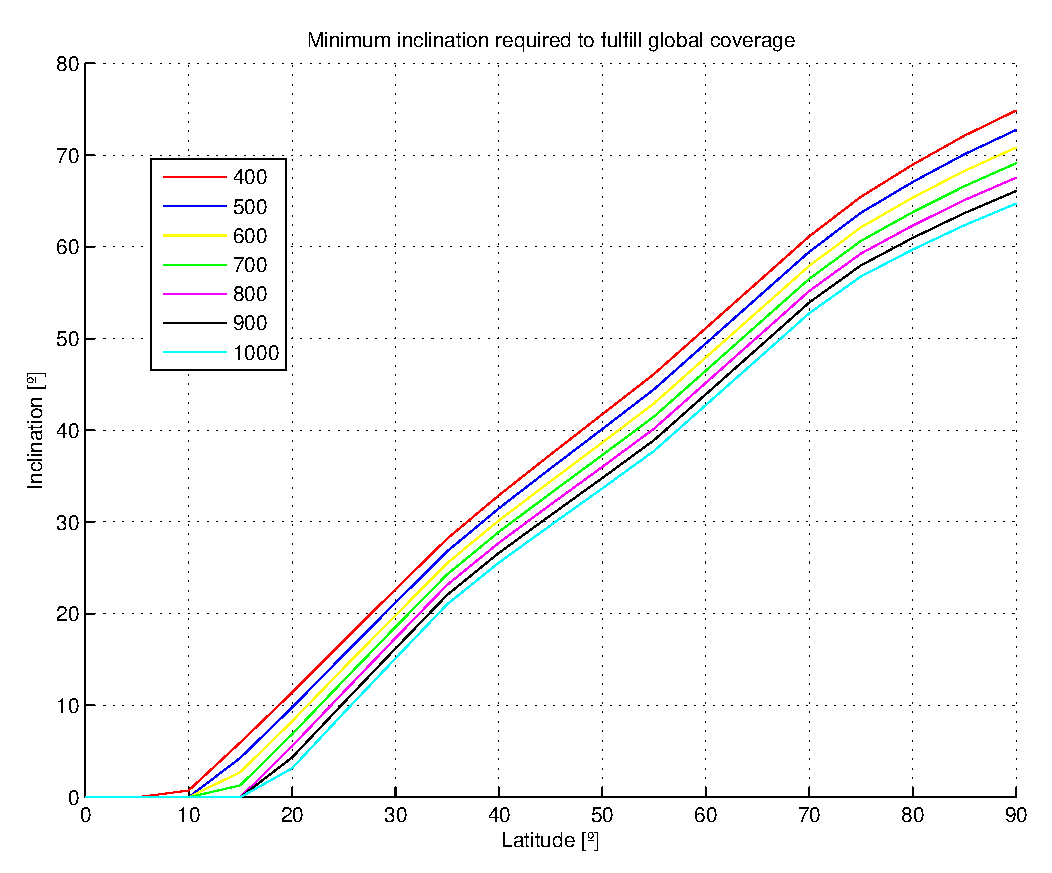
\includegraphics[scale=0.8]{MinimumInclinationPlot}
\caption{Minimum Inclination to provide coverage at different latitude for different orbit apogees.}	
\end{figure}

As it can be observed, if the goal of the design is to provide full global coverage, the distribution of elevation angles with latitude is not significant, since the inclination is required to be higher than approximately 75º. In the other cases, the change of minimum elevation angle distribution causes changes of tendency in the distribution of inclination required. 

\subsubsubsection*{Conclusion}
The main point is that there is a limit inclination for a Walker-Delta constellation configuration in order to provide global coverage at the desired latitude. With this study, this limits in the design algorithms can be set.